% Figure 3: placeholder-contamination test (mechanism of the early-target gain), Qwen3-14B, layer 32, 175 two-word items.
% Numbers verified from runs/w3_B_x3i3_14b_ans_L32 (same, block 4), runs/w5_ph_14b_B_i3 (all<=4, all<=32),
% runs/w5_ph_14b_B_cont and runs/w4_B_x3cont_14b_ans_L32 (continuation prefix rates).
\documentclass[10pt,border=2pt]{standalone}
\usepackage{newtxtext}
\usepackage[T1]{fontenc}
\usepackage{pgfplots}
\pgfplotsset{compat=1.18}
\definecolor{wblue}{HTML}{0072B2}
\definecolor{wgreen}{HTML}{009E73}
\begin{document}
\small
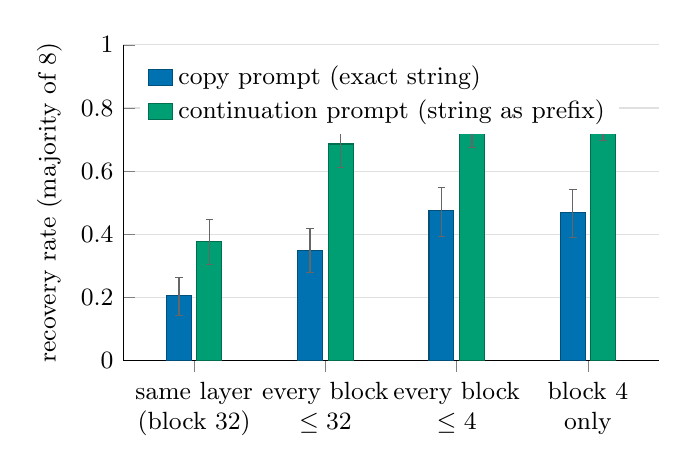
\begin{tikzpicture}
\begin{axis}[
  ybar, width=3.3in, height=2.2in,
  ymin=0, ymax=1.0,
  ylabel={recovery rate (majority of 8)},
  ylabel style={font=\small},
  tick label style={font=\small},
  xtick=data,
  xticklabels={{same layer\\(block 32)},{every block\\$\le 32$},{every block\\$\le 4$},{block 4\\only}},
  xticklabel style={align=center,font=\small},
  bar width=9pt,
  enlarge x limits=0.18,
  legend style={at={(0.03,0.97)},anchor=north west,font=\small,draw=none,fill=white,legend cell align=left},
  legend image code/.code={\draw[#1] (0cm,-0.1cm) rectangle (0.3cm,0.1cm);},
  axis x line*=bottom, axis y line*=left,
  ymajorgrids, grid style={black!12},
  error bars/y dir=both, error bars/y explicit,
  error bars/error bar style={black!60,line width=0.5pt},
  error bars/error mark options={rotate=90,mark size=1.4pt,black!60},
]
\addplot[fill=wblue,draw=wblue!70!black] coordinates {
 (0,0.206) -= (0,0.063) += (0,0.057)
 (1,0.349) -= (0,0.069) += (0,0.068)
 (2,0.474) -= (0,0.080) += (0,0.075)
 (3,0.469) -= (0,0.080) += (0,0.074)
};
\addplot[fill=wgreen,draw=wgreen!70!black] coordinates {
 (0,0.377) -= (0,0.074) += (0,0.069)
 (1,0.686) -= (0,0.075) += (0,0.068)
 (2,0.737) -= (0,0.063) += (0,0.069)
 (3,0.760) -= (0,0.063) += (0,0.069)
};
\legend{copy prompt (exact string), continuation prompt (string as prefix)}
\end{axis}
\end{tikzpicture}
\end{document}
